\documentclass[trans]{beamer}
\usepackage{colortbl}
\usepackage{pgfplots}
\usepackage{subcaption}
\usetheme{CambridgeUS}
\setbeamersize{text margin left=10mm,text margin right=10mm}
\setbeamercovered{invisible}

\input{mathfonts}
% Math essential packages
\usepackage[dvipsnames]{xcolor}
\usepackage{latexsym, mathtools}
\usepackage{amsmath, amssymb, amsfonts, amsthm, amsxtra}
\usepackage[nomathsymbols]{polski}
\usepackage{amscd, tikz-cd}
\usepackage[skip=10pt, indent=0pt]{parskip}
\usepackage[a4paper, left=30mm, right=30mm, top=25mm, bottom=25mm]{geometry}
\usepackage{graphicx, float}
\usepackage[most,many,breakable]{tcolorbox}
\usepackage{relsize}
\usepackage{fancyhdr}
\usepackage{url}
\usepackage[colorlinks=true,citecolor=Periwinkle,urlcolor=Periwinkle,linkcolor=Periwinkle,pdfpagemode=UseNone]{hyperref}

\usepackage[framemethod=TikZ]{mdframed}
\usepackage{thmtools}

\definecolor{accent}{RGB}{163,0,0}
\setlength{\arrayrulewidth}{0.2mm}
% \setlength{\tabcolsep}{1em}
\renewcommand{\arraystretch}{1.2}
% \arrayrulecolor{accent!70}

\title{Regresja Liniowa}
\author{Zachariasz Jażdżewski, Bartosz Guzowzski}
\date{18 maja 2024}

\begin{document}

%----Proper document------------------------------------------------------------

\frame{\titlepage}

\section{Wprowadzenie}

\begin{frame}{Wprowadzenie}
	\onslide<2->
	\begin{table}[!h]
		\begin{tabular}{ ccc }
			\hline
			\bfseries \color{accent} Indeks & \bfseries \color{accent} Dochody & \color{accent} \bfseries Wydatki \\ \hline
			1 & 200 & 120 \\
			2 & 250 & 190 \\
			3 & 285 & 200 \\
			4 & 300 & 270 \\
			5 & 350 & 285 \\
			6 & 395 & 320 \\
			7 & 440 & 340 \\
			8 & 490 & 340 \\
			9 & 510 & 390 \\
			10 & 530 & 410 \\
			\hline
		\end{tabular}
	\end{table}
\end{frame}

\begin{frame}
	\begin{figure}[h!]
		\centering
		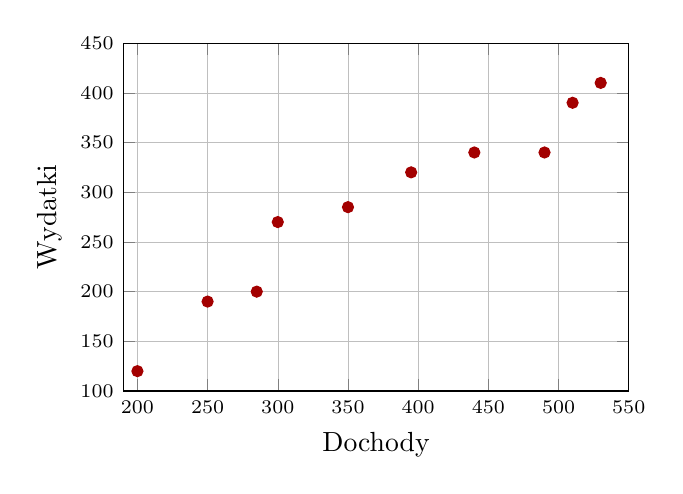
\begin{tikzpicture}
		\begin{axis}[
			xlabel={Dochody},
			ylabel={Wydatki},
			ymin=100, ymax=450,
			xmin=190, xmax=550,
			xtick={200,250,300,350,400,450,500,550},
			ytick={0,50,100,150,200,250,300,350,400,450},
			grid=both,
			grid style={line width=.1pt, draw=gray!10},
			major grid style={line width=.2pt,draw=gray!50},
			width=8cm,
			height=6cm,
			tick label style={font=\scriptsize}
		]
		\addplot[
			only marks,
			color=accent,
			mark=*,
			]
			coordinates {
			(200,120) (250,190) (285,200) (300,270) (350,285) (395,320) (440,340) (490,340) (510,390) (530,410)
			};
		\end{axis}
		\end{tikzpicture}
	\end{figure}
\end{frame}

\begin{frame}
	\onslide<1-> Mamy $n = 10$ obserwacji, które przedstawiamy na płaszczyźnie jako punkty
	\[
		(x_i, y_i) \in \{(200,120),(250,190),...,(530,410)\}, \quad i = 1,2,...,n
	\]
	\begin{itemize}
		\item<2-> Pozytywna korelacja między $\color{accent} x$ a $\color{accent} y$
		\item<3-> Chcemy dopasować krzywą do danych 
		\item<4-> Punkty układają się wzdłuż jakiejś prostej
		\item<5-> Chcemy wybrać najlepszą prostą
		\item<6-> Czym jest ta "najlepsza prosta"?
	\end{itemize}
\end{frame}

\begin{frame}
	\begin{figure}[h!]
		\centering
		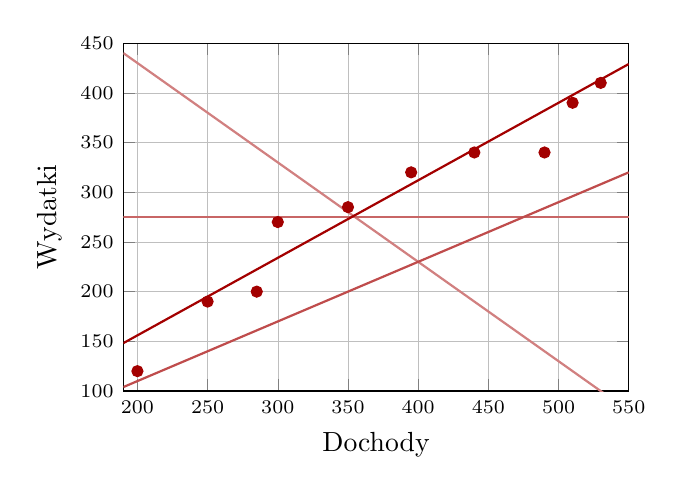
\begin{tikzpicture}
		\begin{axis}[
			xlabel={Dochody},
			ylabel={Wydatki},
			ymin=100, ymax=450,
			xmin=190, xmax=550,
			xtick={200,250,300,350,400,450,500,550},
			ytick={0,50,100,150,200,250,300,350,400,450},
			grid=both,
			grid style={line width=.1pt, draw=gray!10},
			major grid style={line width=.2pt,draw=gray!50},
			width=8cm,
			height=6cm,
			tick label style={font=\scriptsize}
		]
		\addplot[
			only marks,
			color=accent,
			mark=*,
			]
			coordinates {
			(200,120) (250,190) (285,200) (300,270) (350,285) (395,320) (440,340) (490,340) (510,390) (530,410)
			};
		\addplot[
			domain=190:550, 
			samples=100, 
			color=accent!50,
			thick
		]{-x + 630};
		\addplot[
			domain=190:550, 
			samples=100, 
			color=accent!60,
			thick
		]{275};
		\addplot[
			domain=190:550, 
			samples=100, 
			color=accent!70,
			thick
		]{0.6*x - 10};
		\addplot[
			domain=190:550, 
			samples=100, 
			color=accent,
			thick
		]{0.78*x};
		\end{axis}
		\end{tikzpicture}
	\end{figure}
	\begin{itemize}
		\item<2-> Która prosta jest lepsza od innych?
		\item<3-> Dlaczego?
		\item<4-> Potrzebujemy obiektywnej metody!
	\end{itemize}
\end{frame}

\section{Metoda najmniejszych kwadratów}

\begin{frame}{Metoda najmniejszych kwadratów}
	\centering
	\begin{figure}[!h]
		\includegraphics[width=0.35\textwidth]{Carl_Friedrich_Gauss.jpg}
		\caption{Carl Friedrich Gauss}
	\end{figure}
\end{frame}

\begin{frame}
	\begin{itemize}
		\item<1-> Minimalizacja błędu
		\item<2-> Chcemy znaleźć parametry $\color{accent} a$ i $\color{accent} b$
		\item<3-> Różnica między punktami a szacowaną prostą jak najmniejsza 
	\end{itemize}
	\onslide<4->
	\[
		y_i - (\hat a x_i + \hat b) \color{accent} \leftarrow \text{reszta}
	\]
	\onslide<5->
	\[
		\hat a, \hat b \color{accent} \leftarrow \text{estymatory}
	\]
	\begin{itemize}
		\item<6-> Im bliżej estymatory są bliskie prawdziwym parametrom, tym reszta jest mniejsza
	\end{itemize}
\end{frame}

\begin{frame}
	\begin{itemize}
		\item<1-> Zkwadratujmy reszty
		\item<2-> Pozbywamy się problemu ujemnych i dodatnich reszt
	\end{itemize}
	\onslide<3->
	\begin{gather*}
		(y_1 - \hat a x_1 - \hat b)^2 + (y_2 - \hat a x_2 - \hat b)^2 + ... + (y_n - \hat a x_n - \hat b)^2 = \\
		= \sum_{i=1}^n\,(y_i - \hat a x_i - b)^2 \color{accent} \leftarrow \text{suma kwadratów różnic}
	\end{gather*}
	\begin{itemize}
		\item<4-> Suma najmniejsza $\iff$ każda różnica do kwadratu najmniejsza 
	\end{itemize}
\end{frame}

\begin{frame}
	\begin{figure}[h!]
		\centering
		\begin{subfigure}[b]{0.45\textwidth}
			\centering
			\begin{tikzpicture}
			\begin{axis}[
				ymin=100, ymax=450,
				xmin=190, xmax=550,
				xtick={200,300,400,500},
				ytick={200,300,400},
				grid=both,
				grid style={line width=.1pt, draw=gray!10},
				major grid style={line width=.2pt,draw=gray!50},
				width=\textwidth,
				height=\textwidth,
				tick label style={font=\tiny}
			]
			\addplot[
				only marks,
				color=accent,
				mark=*,
				]
				coordinates {
				(200,120) (250,190) (285,200) (300,270) (350,285) (395,320) (440,340) (490,340) (510,390) (530,410)
				};
			\addplot[
				domain=190:550, 
				samples=100, 
				color=accent,
				thick
				]{0.66*x+30};
			\node[anchor=north east] at (axis cs:550,180) {$y = \frac{2}{3}x + 30$};
			\end{axis}
			\end{tikzpicture}
		\end{subfigure}%
		\begin{subfigure}[b]{0.45\textwidth}
			\centering
			\begin{tikzpicture}
			\begin{axis}[
				ymin=100, ymax=450,
				xmin=190, xmax=550,
				xtick={200,300,400,500},
				ytick={200,300,400},
				grid=both,
				grid style={line width=.1pt, draw=gray!10},
				major grid style={line width=.2pt,draw=gray!50},
				width=\textwidth,
				height=\textwidth,
				tick label style={font=\tiny}
			]
			\addplot[
				only marks,
				color=accent,
				mark=*,
				]
				coordinates {
				(200,120) (250,190) (285,200) (300,270) (350,285) (395,320) (440,340) (490,340) (510,390) (530,410)
				};
			\addplot[
				domain=190:550, 
				samples=100, 
				color=accent,
				thick
				]{0.5*x+100};
			\node[anchor=north east] at (axis cs:550,180) {$y = \frac{1}{2}x + 100$};
			\end{axis}
			\end{tikzpicture}
		\end{subfigure}%
	\end{figure}
	\begin{figure}[h!]
		\centering
		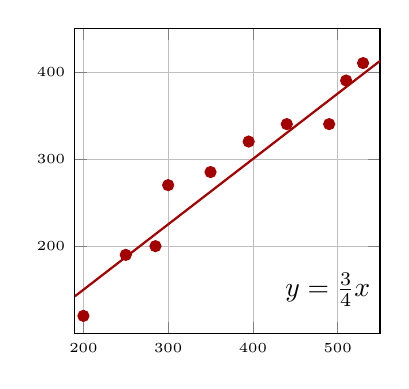
\begin{tikzpicture}
			\begin{axis}[
				ymin=100, ymax=450,
				xmin=190, xmax=550,
				xtick={200,300,400,500},
				ytick={200,300,400},	
				grid=both,
				grid style={line width=.1pt, draw=gray!10},
				major grid style={line width=.2pt,draw=gray!50},
				width=0.45\textwidth,
				height=0.45\textwidth,
				tick label style={font=\tiny}
			]
			\addplot[
				only marks,
				color=accent,
				mark=*,
				]
				coordinates {
				(200,120) (250,190) (285,200) (300,270) (350,285) (395,320) (440,340) (490,340) (510,390) (530,410)
				};
			\addplot[
				domain=190:550, 
				samples=100, 
				color=accent,
				thick
				]{0.75*x};
			\node[anchor=north east] at (axis cs:550,180) {$y = \frac{3}{4}x$};
			\end{axis}
		\end{tikzpicture}
	\end{figure}
\end{frame}

\begin{frame}
	\begin{itemize}
		\item<1-> Dla $\color{accent} y = \frac{2}{3} + 30$ suma kwadratów reszt wynosi $\color{accent} 6\,769.4$
		\item<2-> Dla $\color{accent} y = \frac{1}{2} + 100$ suma kwadratów reszt wynosi $\color{accent} 14\,112.5$
		\item<3-> Dla $\color{accent} y = \frac{3}{4}$ suma kwadratów reszt wynosi $\color{accent} 5\,259.4$
	\end{itemize}
	\onslide<4-> Zatem trzecia linia najlepiej jest dopasowana do danych spośród tej trójki 
\end{frame}

\begin{frame}
		Wzory na parametry najlepszej prostej
		\[
			a = \frac{\sum_{i=1}^n\, y_i(x_i - \bar x)}{\sum_{i=1}^n\, (x_i - \bar x)^2}, \quad b = \bar y - \bar x a
		\]
		gdzie $\overline{x}$ i $\overline{y}$ to średnie arytmetyczne zmiennych $x$ i $y$
\end{frame}

\section{Metoda najmniejszych kwadratów w praktyce}

\begin{frame}{Metoda najmniejszych kwadratów w praktyce}
	Podstawmy nasze dane do wzorów!
	\begin{itemize}
		\item<2-> $\bar x = \frac{1}{10} (200+250+\dots+530)=375$
		\item<3-> $\bar y = \frac{1}{10} (120+190+\dots+200)=286.5$
	\end{itemize}
\end{frame}

\begin{frame}
	Następnie obliczymy odpowiednie sumy do wzoru na \\ współczynnik $a$
	\onslide<2->
	\begin{gather*}
		\sum_{i=1}^{10}\, y_i(x_i - \bar x) = 120 \cdot (200-375) + ... + 410 \cdot (530-375) = 93\,675 \\
		\sum_{i=1}^{10}\, (x_i - \bar x)^2 = (200-375)^2 + ... + (530-375)^2 = 120\,700 \\
	\end{gather*}
\end{frame}

\begin{frame}
	Zostało nam już tylko podstawienie liczb do wzorów na \\ parametry $a$ i $b$
	\begin{itemize}
		\item<2-> $a = \frac{93\,675}{120\,700} \approx 0.78$
		\item<3-> $b = 286.5 - 375 \cdot 0.78 \approx -4.54$
	\end{itemize}
	\onslide<4-> Zatem szukana funkcja jest postaci
	\[
		y = 0.7761x - 4.5367
	\]
\end{frame}

\begin{frame}
	\begin{figure}[h!]
		\centering
		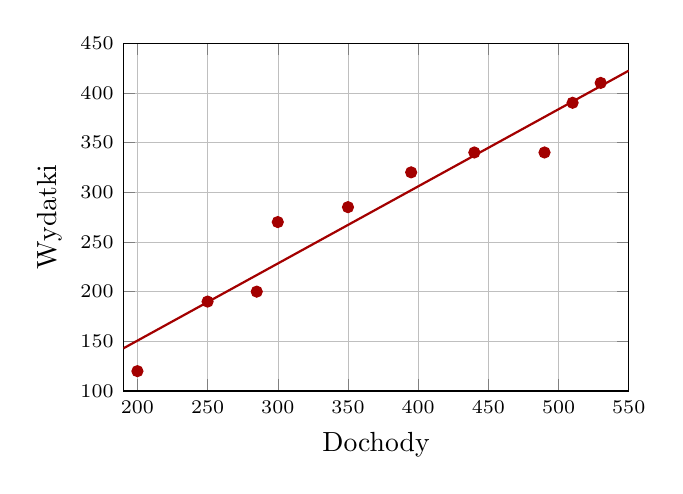
\begin{tikzpicture}
		\begin{axis}[
			xlabel={Dochody},
			ylabel={Wydatki},
			ymin=100, ymax=450,
			xmin=190, xmax=550,
			xtick={200,250,300,350,400,450,500,550},
			ytick={0,50,100,150,200,250,300,350,400,450},
			grid=both,
			grid style={line width=.1pt, draw=gray!10},
			major grid style={line width=.2pt,draw=gray!50},
			width=8cm,
			height=6cm,
			tick label style={font=\scriptsize}
		]
		\addplot[
			only marks,
			color=accent,
			mark=*,
			]
			coordinates {
			(200,120) (250,190) (285,200) (300,270) (350,285) (395,320) (440,340) (490,340) (510,390) (530,410)
			};
		\addplot[
			domain=190:550, 
			samples=100, 
			color=accent,
			thick
			]{0.7761*x - 4.5367};
		\end{axis}
		\end{tikzpicture}
	\end{figure}
	\[
		\sum_{i=1}^n\,(y_i - \hat a x_i - b)^2 = \color{accent} 4901.5
	\]
\end{frame}

\section{Podsumowanie}

\begin{frame}{Podsumowanie}
	\begin{itemize}
		\item<2-> Regresja liniowa to opis korelacji między zmiennymi za pomocą krzywej
		\item<3-> Dopasowanie prostej to znalezienie takich parametrów $a$ i $b$, że funkcja odległości punktów pomiarowych od prostej przyjmuje wartość minimalną
		\item<4-> Metoda najmniejszych kwadratów to takie dopasowanie prostej, aby suma kwadratów różnic między punktami pomiarowymi, a prostą była jak najmniejsza
	\end{itemize}
\end{frame}

\begin{frame}
	Dla zainteresowanych tematem będących ciekawych skąd wzięły się wzory na parametry $a$ i $b$, wykorzystujemy tutaj optymalizację funkcji dwóch zmiennych. Znajdujemy ekstremum lokalne funkcji sumy kwadratów różnic.
\end{frame}

%-------------------------------------------------------------------------------

\end{document}
